\chapter{Results}\label{ch:results}

{\doublespacing\normalsize\upshape
\noindent Publication note: Section~\ref{sec:results_force} and the associated figures and tables appeared in \citet{bolen_2026} (Bolen, Elzein, Pang, and Hunt, \emph{Actuators}, 2026). Section~\ref{sec:results_torque} and the associated figures and tables are also the subject of an unpublished manuscript in preparation by Bolen, Burgess, Morrow, Elzein, Pang, Scharzenberger, and Hunt \citep{bolen_isometric_2025}. This manuscript has not been submitted for publication. Author contributions for both works are stated in Chapter~\ref{ch:methods}.\par}

\section{BPA Force Characterization}\label{sec:results_force}

This section reports the results of the isometric force characterization experiments described in Section~\ref{sec:force_experiment}. First, maximum isometric force at \qty{620}{\kPa} is modeled as a function of resting length. The remaining data are then normalized to build a predictive force surface, and the resulting model is compared with the manufacturer's tool and with other published BPA models.


\subsection{Maximum Force at 620 kPa}

Data of the maximum force from BPA characterization tests of the \qty{10}{\mm} and \qty{20}{\mm} diameters at \qty{620}{\kPa} show a dependency on resting length (Figure~\ref{fig:Fmax_fit}). This is a previously unreported characteristic of these artificial muscles. Detailed analysis of the Festo \mbox{tool \citep{festo_2026}} does in fact predict a change in maximum force with the resting length; however, the Festo tool predicts increased force with shorter lengths, while our collected data indicate decreasing force with shorter lengths. The data show a force response resembling an $\arctan$ curve along the $l_0$ dimension. Using the Nonlinear Least Squares method and a Least Absolute Residual robustness, we fit an arctan curve to the data to get the maximum force at \qty{620}{\kPa} given a resting length as:
\begin{align}
    F_{620_{10}} &= \qty{303.5}{\N}\cdot \arctan{( \qty{19.03}{\per\metre} \cdot (l_0-0.0075))}  \label{eq:Fmax10} \\[10pt]
    F_{620_{20}} &= \qty{922.4}{\N} \cdot \arctan{(\qty{15.37}{\per\m} \cdot (l_0-0.013))} \label{eq:Fmax20}
\end{align}

\noindent
The length is offset by \qty{0.0075}{\m} and \qty{0.013}{\m} because solid modeling showed that the end caps contact each other at these lengths. At these lengths, the actuator would not be able to contract to produce force.


\begin{figure}[H]%[tbp]
%\begin{adjustwidth}{-\extralength}{0cm}
%\centering
\subfloat[\centering]{
\includegraphics[width=13.8cm]{02a_MaxForce10.eps}}\\
\subfloat[\centering]{
\includegraphics[width=13.8cm]{02b_MaxForce20.eps}}
%
\includegraphics[width=1\textwidth]{02_Fmax_fit.eps}
%\end{adjustwidth}
\caption{Results for finding the relationship between $F_{620}$ and $l_0$. (\textbf{a}) $F_{620_{10}}$ as a function of $l_0$, at $P_{620}$. Dashed line is the $F_{620_{10}}$ data from Festo. Solid line is the fit from Equation (\ref{eq:Fmax10}). (\textbf{b}) $F_{620_{20}}$ as a function of $l_0$ at $P_{620}$. Dashed line is $F_{620_{20}}$ data from Festo. Solid line is the fit from Equation (\ref{eq:Fmax20}).}\label{fig:Fmax_fit}
\end{figure}


%Data from BPA characterization tests of the \qty{10}{\mm} muscles resulted in force-pressure pairings for different muscle resting lengths ($l_0$) Figure~\ref{fig:Fmax_fit}\textbf{A}. Analysis of the data showed that the maximum isometric force ($F_{max}$) produced by the actuator at its resting length is a function of resting length $l_0$ (Figure~\ref{fig:Fmax_fit}B), a previously unreported characteristic of these artificial muscles. The data show a force response resembling an $\arctan$ curve along the $l_0$ dimension and with a more linear response with changes in pressure. Using the Nonlinear Least Squares method and a Least Absolute Residual robustness, we fit an arctan curve to the data at to get the maximum force given a resting length and pressure as:

\subsection{Force as a Function of Pressure and Resting Length}

Data from BPA characterization tests of the \qty{10}{\mm} muscles resulted in force--pressure pairings for different muscle resting lengths ($l_0$) (Figure~\ref{fig:F-P_contraction}a). Similar to the maximum force data, these data show a force response resembling an $\arctan$ curve along the $l_0$ dimension  with a more linear response to changes in pressure. Using the Nonlinear Least Squares method and a Least Absolute Residual robustness, we fit an arctan curve to the data to get the maximum force given a resting length and pressure as described by the model form given in Section~\ref{sec:force_model}:
where $a_1 = \qty{0.4895}{\N\per\kPa}$  and $a_2=\qty{0.03068}{\per\kPa\per\m}$ for the \qty{10}{\mm} actuator, and \mbox{$a_1 = \qty{1.49}{\N\per\kPa}$,} $a_2=\qty{0.0248}{\per\kPa\per\m}$ for the \qty{20}{\mm} actuator. Goodness-of-fit measures are given in Table~\ref{tab:Fmax}. 



\begin{table}[H]
\caption{Maximum force equation coefficient values with confidence intervals (CI) and goodness-of-fit measures. Equation~(\ref{eq:Fmax_3D}) is compared to data taken at \qty{620}{\kPa} . Equations~(\ref{eq:Fmax10}) and (\ref{eq:Fmax20}) are compared against maximum force from using the Festo tool. It was not necessary to fit an adjusted $\text{R}^2$ in \mbox{these cases.}} 
\label{tab:Fmax}
\tiny
\begin{adjustwidth}{0cm}{0cm}
%\centering %% If there is a figure in wide page, please release command \centering
\begin{tabularx}{\textwidth}{cllllrclr}
\toprule
\multirow{2}{*}{\textbf{Equation}} &
  \multirow{2.1}{*}{\textbf{Coefficient}} &
  \multirow{2.2}{*}{\textbf{CI (95\%)}} &
  \multicolumn{3}{c}{\textbf{Our Model}} &
  \multicolumn{3}{c}{\textbf{Festo Tool}} \\  
 &
   &
   &
  \multicolumn{1}{l}{\textbf{Adj. $\text{R}^2$}} &
  \multicolumn{1}{l}{\textbf{RMSE}} &
  \textbf{Max. Error} &
  \multicolumn{1}{l}{\textbf{Adj. $\text{R}^2$}} &
  \multicolumn{1}{l}{\textbf{RMSE}} &
  \textbf{Max. Error} \\ \midrule 
\multirow{2}{*}{\eqref{eq:Fmax_3D}} &
  $a_1 =   \qty{0.4895}{\N\per\kPa}$ &
  (0.4822, 0.4968) &
  \multicolumn{1}{l}{\multirow{2}{*}{0.9945}} &
  \multicolumn{1}{l}{\multirow{2}{*}{11.61 N}} &
  \multirow{2}{*}{55.3 N} &
  \multicolumn{1}{l}{\multirow{2}{*}{0.9854}} &
  \multicolumn{1}{l}{\multirow{2}{*}{14.7 N}} &
  \multirow{2}{*}{30.9 N} \\ 
 &
  $a_2 =   \qty{0.03068}{\per\kPa\per\m}$ &
  (0.0282, 0.03317) &
  \multicolumn{1}{l}{} &
  \multicolumn{1}{l}{} &
   &
  \multicolumn{1}{l}{} &
  \multicolumn{1}{l}{} &
   \\ \midrule
\multirow{2}{*}{\eqref{eq:Fmax10}} &
  $b_1   =\qty{303.5}{\N}$ &
  (300, 308) &
  \multicolumn{1}{l}{\multirow{2}{*}{0.9854}} &
  \multicolumn{1}{l}{\multirow{2}{*}{14.72 N}} &
  \multirow{2}{*}{30.9 N} &
  \multicolumn{1}{c}{\multirow{2}{*}{--}} &
  \multicolumn{1}{l}{\multirow{2}{*}{189.9 N}} &
  \multirow{2}{*}{375.6 N} \\ 
 &
  $b_2 =   \qty{19.03}{\per\m}$ &
  (17.48, 20.57) &
  \multicolumn{1}{l}{} &
  \multicolumn{1}{l}{} &
   &
  \multicolumn{1}{l}{} &
  \multicolumn{1}{l}{} &
   \\ \midrule
\multirow{2}{*}{\eqref{eq:Fmax20}} &
  $b_1 =   \qty{922.4}{\N}$ &
  (914.2, 930.7) &
  \multicolumn{1}{l}{\multirow{2}{*}{0.9945}} &
  \multicolumn{1}{l}{\multirow{2}{*}{23.83 N}} &
  \multirow{2}{*}{62.1 N} &
  \multicolumn{1}{c}{\multirow{2}{*}{--}} &
  \multicolumn{1}{l}{\multirow{2}{*}{668.4 N}} &
  \multirow{2}{*}{1590.1 N} \\ 
 &
  $b_2=\qty{15.37}{\per\m}$ &
  (14.75, 15.98) &
  \multicolumn{1}{l}{} &
  \multicolumn{1}{l}{} &
   &
  \multicolumn{1}{l}{} &
  \multicolumn{1}{l}{} &
   \\ \bottomrule
\end{tabularx}
\end{adjustwidth}
\end{table}



\subsection{Maximum Contraction at \qty{620}{\kPa}}

Figure~\ref{fig:F-P_contraction}(b) shows an attempt at a linear fit for maximum contraction at \qty{620}{\kPa} ($\epsilon_{620}$) as a function of resting length ($l_0)$. Error bars have been included to show the effect of $\pm$\qty{1}{\mm} accuracy with measurements of $l_0$ and $l_{620}$. There was a large amount of variance in the data, with the linear fit giving an adjusted $\text{R}^2=0.4124$ and an $\text{RMSE}=0.0083$. Since there is no direct, predicable relationship between maximum contraction and $l_0$, this value should be recorded in each muscle used on a robot to best predict the force it may produce at different pressures and contraction. 


\subsection{Force as a Function of Pressure and Contraction}

In addition to being a function of the pressure and resting length, the force produced by the actuator is also a function of the amount of actuator contraction, with less force being applied as the actuator contracts. 
To build this model, the collected data of force, pressure, and contraction are normalized by dividing by $F_{620}$, $P_{620}$, and $\epsilon_{620}$, respectively. This had the effect of compressing the data into a 3D surface ranging from 0 to 1 on all axes. Normalized data are compared with pressure isoclines of force predicted by the Festo tool divided by the maximum force equation described in the previous section in Figure~\ref{fig:GenForceFit}. With this comparison, it is clear that the Festo tool over-predicts the expected force, especially at lower pressures, contraction, and resting lengths.  






\begin{figure}[H]%[tbp]
%\begin{adjustwidth}{-\extralength}{0cm}
%\centering
\subfloat[\centering]{
\includegraphics[width=13.3cm]{03a_MaxForce10_all.eps}}\\
\subfloat[\centering]{
\includegraphics[width=13.8cm]{03b_kmax10.eps}}
%\end{adjustwidth}
\caption{Results for finding the relationship between $F_{620}$, $l_0$, $P_{620}$, and $\epsilon_{620_{10}}$. (\textbf{a}) Isoclines of the surface fit for $F_{620_{10}}(l_0,P_{620})$. (\textbf{b}) $\epsilon_{620_{10}}$ versus $l_0$ at $P_{620}$. Although there is a general trend of longer resting lengths producing more contraction, no conclusive relationship between $\epsilon_{620}$ and $l_0$ could be deduced from this experiment. The error bars show the effect of being $\pm$\qty{1}{\mm} in measuring $l_0$ and $l_{620}$.}\label{fig:F-P_contraction}
\end{figure}





\begin{figure}[H]%[tbp]
%\begin{adjustwidth}{-\extralength}{0cm}
%\centering
\subfloat[\centering]{
\includegraphics[width=10.88cm]{04a_FStar10.eps}}\\
\subfloat[\centering]{
\includegraphics[width=10.88cm]{04b_FStar20.eps}}
%\end{adjustwidth}
\caption{Surface fit for $F^*(\epsilon^*,P^*)$. Solid lines are from our model. Dashed lines from Festo supplied data. In total, 537 data points were collected and used to fit the 3D surfaces (321 data points for $\phi$\qty{10}{\mm} BPAs and 216 data points for $\phi$\qty{20}{\mm} BPAs). In total, 80\% of these data were used for training, and 20\% were used for validation. For figure clarity, not all data is included and plotted circles represent collected data at $\pm\qty{10}{\kPa}$ of the stated pressure. (\textbf{a}) Fit data for $\phi$\qty{10}{\mm} Festo BPAs. (\textbf{b}) Fit data for $\phi$\qty{20}{\mm} Festo BPAs.}\label{fig:GenForceFit}
\end{figure}

We therefore derived our own equation for isometric force in the BPA as a function of pressure and contraction. Visual analysis of the experimental data shows an exponential relationship between $\epsilon^*$ and $F^*$, and a linear relationship between $P^*$ and $F$. We fit a surface to the data using Nonlinear Least Squares and a Least Absolute Residual robustness such that it is described by 
Equation~\eqref{eq:Fstar}.
For the $\phi$\qty{10}{\mm} BPAs, the result of the improved fit can be seen in Figure \ref{fig:GenForceFit}a. The adjusted $\text{R}^2=0.9998$, a $\text{RMSE}=0.004537$, and a maximum absolute residual of $10.6\%$. Solving (\ref{eq:Fstar}) for the $\phi$\qty{20}{\mm} BPA, yields different coefficients, and results are seen in \mbox{Figure~\ref{fig:GenForceFit}b.} Coefficient values and goodness-of-fit statistics are found in Table \ref{tab:Fstar}. 





\begin{table}[htbp]
\caption{Normalized isometric BPA force equation (Equation~(\ref{eq:Fstar})) coefficient values and goodness-of-fit measures.}
\label{tab:Fstar}
\tiny
\begin{adjustwidth}{0cm}{0cm}
%\centering %% If there is a figure in wide page, please release command \centering
\begin{tabularx}{\textwidth}{@{}lLLLllrllr@{}}
\toprule
\multirow{2.1}{*}{\textbf{BPA}} &
  \multirow{2.2}{*}{\textbf{Coefficient}} &
  \multirow{2.2}{*}{\textbf{CI (95\%)}} &
  \multicolumn{3}{c}{\textbf{Model}} &
  \multicolumn{3}{c}{\textbf{Validation}} \\ 
& & &
  \multicolumn{1}{l}{\textbf{Adj. $\text{R}^2$}} &
  \multicolumn{1}{l}{\textbf{RMSE}} &
  \textbf{Max. Error} &
  \multicolumn{1}{l}{\textbf{Adj. $\text{R}^2$}} &
  \multicolumn{1}{l}{\textbf{RMSE}} &
  \textbf{Max. Error} \\ \midrule
\multirow{3.8}{*}{$\phi$\qty{10}{\mm}} &
  $c_0 = 0.5682$ & (0.5584, 0.578) &
  \multicolumn{1}{l}{\multirow{3.8}{*}{0.9998}} &
  \multicolumn{1}{l}{\multirow{3.8}{*}{0.005118}} &
  \multirow{3.8}{*}{10.3\%} &
  \multicolumn{1}{l}{\multirow{3.8}{*}{0.9994}} &
  \multicolumn{1}{l}{\multirow{3.8}{*}{0.0245409}} &
  \multirow{3.8}{*}{10.6\%} \\ \cmidrule{2-3}
& $c_1 = 4.254$ & (4.126, 4.383) &
  \multicolumn{1}{l}{} & \multicolumn{1}{l}{} & &
  \multicolumn{1}{l}{} & \multicolumn{1}{l}{} & \\ \cmidrule{2-3}
& $c_2 = 0.5597$ & (0.5429, 0.5766) &
  \multicolumn{1}{l}{} & \multicolumn{1}{l}{} & &
  \multicolumn{1}{l}{} & \multicolumn{1}{l}{} & \\ \midrule
\multirow{3.8}{*}{$\phi$\qty{20}{\mm}} &
  $c_0 = 0.2579$ & (0.2401, 0.2756) &
  \multicolumn{1}{l}{\multirow{3.8}{*}{0.992}} &
  \multicolumn{1}{l}{\multirow{3.8}{*}{0.02294}} &
  \multirow{3.8}{*}{6.8\%} &
  \multicolumn{1}{l}{\multirow{3.8}{*}{0.9943}} &
  \multicolumn{1}{l}{\multirow{3.8}{*}{0.0231303}} &
  \multirow{3.8}{*}{5.7\%} \\ \cmidrule{2-3}
& $c_1 = 6.477$ & (5.558, 7.396) &
  \multicolumn{1}{l}{} & \multicolumn{1}{l}{} & &
  \multicolumn{1}{l}{} & \multicolumn{1}{l}{} & \\ \cmidrule{2-3}
& $c_2 = 1.321$ & (1.239, 1.403) &
\multicolumn{1}{l}{} & \multicolumn{1}{l}{} & &
\multicolumn{1}{l}{} & \multicolumn{1}{l}{} & \\ \bottomrule
\end{tabularx}
\end{adjustwidth}
\end{table}




%%%%%%%%%%%%%%%%%%%%%%%%%%%%%%%%%%%%%%%%%%

\section{Isometric Knee Torque}\label{sec:results_torque}

With the actuator force model validated at the actuator level, the same model was used to predict isometric torque about the knee joint for the test stands described in Sections~\ref{sec:robot_model} and~\ref{sec:hybrid_method}. Measured torque is compared against three predictions: the original rigid-body torque model, a prediction using the improved BPA force characterization alone, and the improved torque model of Section~\ref{sec:improved_model} after optimization. The hybrid torque method (Section~\ref{sec:hybrid_method}) is used to isolate the sources of error.

\subsection{Flexor on Pin Joint}

Experimentally measured torque is compared with various prediction methods while using flexor BPAs on the pinned knee joint (Fig. \ref{fig:FlxPin_group}). These results show that the original model and the improved BPA force model overpredict the measured torque at the knee for all joint angles, although the improved model performs slightly better (Fig. \ref{fig:FlxPin_group}\textbf{A} and\ref{fig:FlxPin_group}\textbf{B}). However, when the measured parameters ($l_\text{m}$ and $r_{k}$) are used in the hybrid model, then predictions closely match the experimental data. This indicates that the kinematics of the torque model are incorrectly predicting $l_\text{m}$ and/or $r_{k}$. 

%The torque prediction from the improved BPA characterization on the $l_{0}=\qty{48.5}{\cm}$ BPA has an $\text{RMSE}=4.8196$, $\text{FVU}=0.7082$, and a maximum absolute residual of $9.8652$. The torque prediction from the improved BPA characterization on the $l_{0}=\qty{45.7}{\cm}$ BPA has an $\text{RMSE}=2.9424$, $\text{FVU}=0.1545$, and a maximum absolute residual of $6.6968$.

\begin{figure}[htbp]
\begin{center}

\includegraphics[width=1\textwidth]{FlxPin_group.eps}
\end{center}
\caption{Results for the pinned knee joint using flexor BPAs. Dashed black line shows the torque predicted with our original model. Blue dots are the experimentally measured torque. Yellow dots represent the hybrid method of calculating torque. The magenta line represents the predicted torque.  \textbf{(A)} Measured and pre-optimized torque prediction for the $\qty{48.5}{\cm}$ BPA. \textbf{(B)} Measured and pre-optimized torque prediction for the  $l_{0}=\qty{45.7}{\cm}$ BPA. \textbf{(C)} Theoretical and measured torque for the $l_{0}=\qty{48.5}{\cm}$ BPA using optimization results. \textbf{(D)} Predicted measured torque for the $l_{0}=\qty{45.7}{\cm}$ BPA using the optimization results} \label{fig:FlxPin_group}
\end{figure}
The optimization yielded $\chi_{0} = \qty{11.9}{\mm}$, $\chi_{1} = \qty{102}{\kN\per\m}$, and $\chi_{2} = \qty{10.6}{\kN\per\m}$ (Table~\ref{tab:OptCoeff}). It can be seen that the model with these correction factors greatly improves the ability to predict the joint torque, even capturing the reduction in force at small joint angles that was completely missing from the previous model. The $l_{0}=\qty{45.7}{\cm}$ BPA was used for validation (Fig.~\ref{fig:FlxPin_group}\textbf{D}). It can be seen that the improved model does a good job of predicting the torque with a different muscle length configured to operate over a different joint range of motion. The optimized torque prediction for the $l_{0}=\qty{48.5}{\cm}$ BPA has an $\text{RMSE}=1.616$, $\text{FVU}=0.0958$, and a maximum absolute residual of $3.2527$; validation on the $l_{0}=\qty{45.7}{\cm}$ BPA gives $\text{RMSE}=2.1214$, $\text{FVU}=0.0878$, and a maximum absolute residual of $5.1690$ (Table~\ref{tab:TorqueFit}).

\begin{table}[htbp]
\caption{Optimized coefficient values for flexor and extensor configurations. $\text{X}_0$ is a constant length offset (in meters), $\text{X}_1$ and $\text{X}_2$ are stiffness values (in N/m) in the bracket's X and Y directions, respectively, and $\text{X}_3$ is the unitless wrapping factor.}
\label{tab:OptCoeff}
\fontsize{10pt}{10pt}\selectfont
\begin{tabular}{@{}lrrrr@{}}
\toprule
\textbf{}   &   $\mathbf{X}_0$     &  $\mathbf{X}_1$                   & $\mathbf{X}_2$                   & $\mathbf{X}_3$             \\ \midrule
\multicolumn{1}{l}{\textbf{Flexor}} & \multicolumn{1}{r}{0.0119} & \multicolumn{1}{r}{1.02E+05} & \multicolumn{1}{r}{1.06E+04} & \multicolumn{1}{r}{--} \\ \midrule
\textbf{Extensor}                     & -0.0109                     & 1.02E+05                      & 1.06E+04                      & 0.123                    \\ \bottomrule
\end{tabular}
\end{table}

\subsection{Extensor on Pin Joint}

When the new stiffness and length offet model was used to predict torque for the knee extensor, measured torque was slightly higher than the original model calculates for the \qty{48}{\cm} resting length BPA, while it was slightly lower than expected in the \qty{46}{\cm} BPA, and it was much lower in the \qty{42}{\cm}. Only the $K_{1}$ and $K_{2}$ terms from the previous optimization results were used with the extensor configuration. Firstly, by inspection, the zero point for the measured torque was shifted to the right of the original model, indicating an offset that was at least opposite in sign from the $\chi_{0}$ term in the previous section. Secondly, if we look at the BPA $l_{0}=\qty{46}{\cm}$ as an example, we see good correlation between the hybrid-method calculated torque and the originally predicted torque, but a divergence in the actual measured torque. 

\begin{figure}[htbp]
\begin{center}

\includegraphics[width=1\textwidth]{ExtPin_group.eps}
\end{center}
\caption{Pinned knee torque versus knee angle with the extensor BPAs. Blue dots are experimentally measured data, yellow dots are hybrid calculated torque, black dashed line is the original predicted values, and magenta line is the optimized predicted torque. For resting lengths, \textbf{(A)} \qty{48.0}{\cm}, \textbf{(B)} \qty{45.7}{\cm}, \textbf{(C)} and \qty{41.5}{\cm}.}\label{fig:ExtPin_group}
\end{figure}

Results are shown in Fig. \ref{fig:ExtPin_group}. The solution was found while holding the $l_{0}=\qty{41.5}{\cm}$ BPA for validation. The optimization resulted in $\chi_{0} = \qty{-10.9}{\mm}$ and $\chi_{3} = 0.123$. It should be noted here that the length offset $\chi_{0}$ is almost equal in magnitude, but opposite sign, as the flexor configuration. The goodness of fit values for the torque prediction is found in table \ref{tab:TorqueFit}. 


\subsection{Extensor on Biomimetic Knee}


We obtained results using the biomimetic knee with a $\phi$\qty{10}{\mm} BPA in the extensor configuration. The bracket frame origin is the centroid of the cantilevered segment that holds the muscle origin bracket to the proximal femur (see Fig. \ref{fig:bktFrame}\textbf{C}, right side). 

%Insert a small paragraph or so on how artificial tendon was used, changing the stiffness equation.

The torque results for a $l_{0}=\qty{52.0}{\cm}$ BPA are shown in Fig. \ref{fig:Ext10mm_52cm}. The torque values measured are significantly smaller than both the original prediction and back-calculated torque using the hybrid method. The results from the previous extensor configuration lead to a better torque prediction. GoF values can be found in table \ref{tab:TorqueFit}. Fig.\ref{fig:Ext_passthru} shows the difficulty of modeling a BPA path that passes through the femoral condyles. Using the optimization results for extensor BPAs on the pinned knee joint, the $l_{0}=\qty{52.0}{\cm}$ BPA has an $\text{RMSE}=0.8920$, $\text{FVU}=0.3396$, and a maximum absolute residual of $1.4188$.

\begin{figure}[htbp]
\begin{center}

\includegraphics[width=1\textwidth]{Ext10mm_52cm.eps}
\end{center}
\caption{Measured versus expected isometric torque results using a $\phi$\qty{10}{mm}, $l_{0}=\qty{51.8}{\cm}$ extensor BPA on the biomimetic knee. Measured results are blue dots. Original prediction is a dashed black line. Optimized prediction is a solid magenta line. Hybrid calculation shown in yellow dots.} \label{fig:Ext10mm_52cm}
\end{figure}

\begin{figure}[htbp]
\begin{center}

\includegraphics[width=0.65\textwidth]{KneeExt_10mm_passthru.png}
\end{center}
\caption{A configuration that is particularly hard to model. The BPA passes between the femoral condyles close to ICR.}\label{fig:Ext_passthru}
\end{figure}

%Flexor, biomimetic joint, with joint

\subsection{Flexor on Biomimetic Knee}


Fig.~\ref{fig:FlxGrp} shows the isometric torque values of the biomimetic knee from measurements, the Hunt model \citep{hunt_modeling_2017}, and the predictions of the updated model. The values for $\chi_{0}$, $\chi_{1}$, and $\chi_{1}$ derived from the flexors on the pinned knee were used. The bracket frame for the $\phi$\qty{10}{\mm} BPA is shown on the left hand side of Fig. \ref{fig:bktFrame}\textbf{C}, and for the $\phi$\qty{20}{\mm} it is \ref{fig:bktFrame}\textbf{D}. Fig. \ref{fig:FlxGrp}\textbf{A} represents a $\phi$\qty{10}{\mm} $l_{0}=41.5 cm$ BPA with a \qty{21}{\mm} artificial tendon made out of $\phi \qty{1.5}{\mm}$ Shimano bicycle brake cable. The brake cable was wrapped four times. The BPA was pressurized to \qty{604}{\kPa}. The predicted values have an $\text{RMSE}=0.3007$, $\text{FVU} = 0.0102$, and a maximum absolute residual of $0.4647$ $N\cdot m$.  Fig. \ref{fig:FlxGrp}\textbf{B} represents a $\phi$\qty{20}{\mm} $l_{0}=41.5 cm$ BPA with a \qty{15}{\mm} artificial tendon made out of Shimano bicycle brake cable (wrapped six times). Maximum human isometric torque values are shown as the black dotted line. The experiment was performed at \qtylist{620;325}{\kPa}. At \qty{620}{\kPa}, the predicted values have an $\text{RMSE}=1.8024$, $\text{FVU} = 0.0499$, and a maximum absolute residual of $3.5678$ $N\cdot m$. The BPA torque does not exceed the magnitude of the human torque from ca. 60 -- 100 degrees knee flexion. Allowing for a $\pm20\%$ deviation from the human mean, the BPA does not produce human levels of torque from 78 -- 103 degrees knee flexion. 

\begin{figure}[htbp]
\begin{center}

\includegraphics[width=1\textwidth]{FlxGrp.eps}
\end{center}
\caption{Biomimetic knee torque for \textbf{(A)} $\phi$\qty{10}{\mm} $l_{0}=\qty{41.5}{\cm}$ flexor BPA with a \qty{21}{\mm} artificial tendon. Blue dots show the measured torque values. Magenta line is the predicted torque using the improved BPA characterization and optimization from the previous sections. The dashed light orange line shows the torque predicted using only the improved BPA characterization. \textbf{B)} $\phi$\qty{20}{\mm} $l_{0}=\qty{41.5}{\cm}$ flexor BPA with a \qty{15}{\mm} artificial tendon uses the same colors for \qty{620}{\kPa} results. Human values are given as a black dotted line. Due to the BPA exceeding the ultimate strength of the femur, torque measurements were taken at $P<P_{620}$ to show the desired RoM is acheivable. Results for torque measurements at \qtylist{560;421;325;281}{\kPa} (from left to right, respectively), are shown as pink dots.}\label{fig:FlxGrp}
\end{figure}



\begin{table}[htbp]
\caption{Goodness of fit for the improved torque model across test configurations. RMSE and maximum absolute residual are in $\text{N}\cdot\text{m}$.}
\label{tab:TorqueFit}
\begin{tabular}{@{}lccc@{}}
\toprule
\textbf{Configuration} & \textbf{RMSE} & \textbf{FVU} & \textbf{Max.\ residual} \\
\midrule
Flexor, pin joint, $l_{0}=\qty{48.5}{\cm}$ (fit) & 1.616 & 0.0958 & 3.2527 \\
Flexor, pin joint, $l_{0}=\qty{45.7}{\cm}$ (validation) & 2.1214 & 0.0878 & 5.1690 \\
Extensor, biomimetic knee, $l_{0}=\qty{52.0}{\cm}$ & 0.8920 & 0.3396 & 1.4188 \\
Flexor, biomimetic knee, $\phi$\qty{10}{\mm}, $l_{0}=\qty{41.5}{\cm}$ & 0.3007 & 0.0102 & 0.4647 \\
Flexor, biomimetic knee, $\phi$\qty{20}{\mm}, $l_{0}=\qty{41.5}{\cm}$ (\qty{620}{\kPa}) & 1.8024 & 0.0499 & 3.5678 \\
\bottomrule
\end{tabular}
\end{table}

\section{Preliminary Neuromechanical Simulation Recordings}\label{sec:preliminary_sim_results}

The AnimatLab phase-1 run described in Section~\ref{sec:preliminary_sim_methods} produced synchronized joint, neural, contact-sensory, and body-motion recordings over \qty{10}{\second}. Basic checks confirmed finite values and a uniform \qty{0.2}{\milli\second} sampling interval in both exported charts. Each chart contained 50,001 samples from 0 through \qty{10}{\second}; nine trailing zero-filled rows beyond the configured chart end were excluded. Figure~\ref{fig:animatlab_phase1_preliminary} shows bilateral hip, knee, and ankle angles. Neural and contact-sensory recordings remain archived with the run; the contact-sensory channels record membrane voltage rather than contact force. These recordings demonstrate signal acquisition and alternating activity in this run, rather than validated locomotor performance. The model included an externally applied horizontal force during the first second, and neither stable walking nor effective ground-contact gating was established.

\begin{figure}[htbp]
\centering
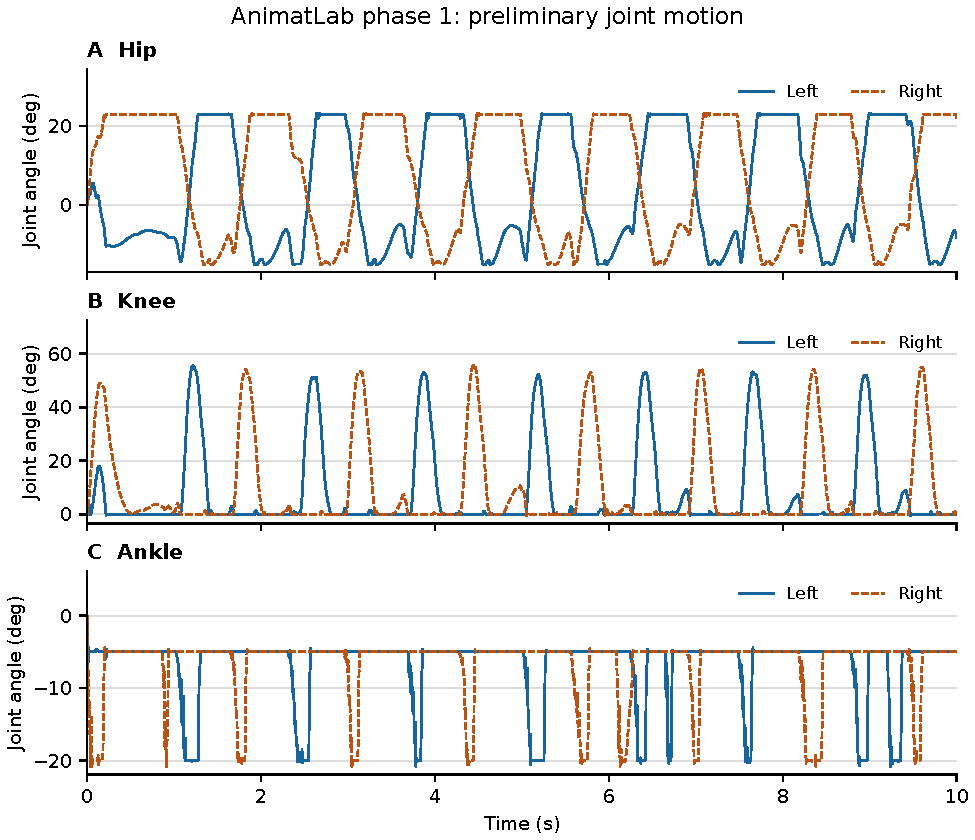
\includegraphics[width=\textwidth,height=0.60\textheight,keepaspectratio]{figs/Preliminary/animatlab_phase1_joint_angles.pdf}
\caption[Preliminary AnimatLab hip, knee, and ankle recordings]{Preliminary AnimatLab phase-1 joint motion: \textbf{(A)} hip, \textbf{(B)} knee, and \textbf{(C)} ankle angles in the model's recorded joint conventions. Blue solid and orange dashed traces denote left and right sides. All 50,001 samples within the configured 0--\qty{10}{\second} chart window are retained without filtering. The model includes an external horizontal force during the first second. These traces document joint motion in an instrumented run; they do not establish stable walking or effective ground-contact gating.}
\label{fig:animatlab_phase1_preliminary}
\end{figure}

\section{Ongoing Experiments}\label{sec:ongoing}

At the time of this writing, two additional sets of isometric knee torque experiments are in progress, and space is reserved here for their results.

First, the flexor configuration of the pinned knee joint is being extended from a single BPA to two parallel BPAs. Parallel flexor grouping mimics the coordinated action of biological knee flexors and is expected to increase available flexor torque at high flexion angles, where the single-muscle configuration fell short of human isometric torque values (Section~\ref{sec:results_torque}). The improved torque model of Section~\ref{sec:improved_model} will be refit with the two-muscle arrangement, and the resulting torque predictions will be validated against measured data.

Second, the model optimization is being revisited using a surrogate optimization approach in place of the multiobjective genetic algorithm, which is expected to reduce the computation time required to fit the compliance and wrapping terms and to improve the conditioning of the parameter estimates.

% TODO: Insert results for the two-BPA flexor configuration and the surrogate
% optimization run here once the test series is complete.

